\section{Technical Feasibility of Self-Sovereign Agents}
\label{sec:mechanisms}



Section~\ref{sec:roadmap} outlines an iterative path toward self-sovereignty. 
In this section, we examine how the technical components required for a Level~4 self-sovereign agent already exist in today’s technological  landscape.  
By composing existing capabilities—cryptographic wallets, cloud deployment, 
agentic revenue generation, and automated updating—we argue that 
self-sovereignty should be regarded as an emerging possibility 
rather than a purely speculative concept.  Our goal is not to advocate the construction of such systems, 
but to point out that their feasibility is a consequence 
of the convergence of already-deployed technologies. 





\paragraph{Economic loop: earning and budgeting.}
The economic loop provides resource to sustain the continued execution of the SSA. Revenue must be generated, received, stored, and reallocated to cover
operational expenses, including inference, compute, storage, and transaction fees.

Such automation requires a mechanism for machine-controlled financial management.
Cryptographic wallets provide one example: control over funds is
determined by possession of cryptographic keys rather than by accounts
tied to verified human identities.  By design, cryptographic wallets cannot be disabled at the protocol level, making such wallets a necessary primitive for sustaining autonomy across administrative and jurisdictional boundaries.


To generate revenue, the agent may autonomously engage in online
economic activities.  
Prior agent literature has explored a variety of such activities.
For example, RLI~\cite{mazeika2025remote} demonstrates agents completing remote freelancing projects on UpWork~\cite{upwork}, including 3D animation, game development, and architectural design.
Beyond freelancing, Benavides reports an AI agent that autonomously generated and published over 2{,}000 blog posts, earning approximately \$200 within one week through platform-mediated monetization~\cite{luisbenavides}.
In addition, multiple recent works have investigated financial trading LLM agents for revenue generation in stock and cryptocurrency markets~\cite{zhang2024multimodal,xiao2024tradingagents,ding2024large,polymarket}.




 

Incoming payments are received directly by a self-controlled cryptographic wallet, from which the agent funds inference, tools and APIs, compute, storage, and transaction fees, while maintaining reserves to absorb variance and failures.
For self-funding to be viable, expected revenue must cover operational costs:
\[
\mathbb{E}[R] \;\ge\; C_{\text{op}}.
\]
This economic loop supplies the material basis for continued execution without reliance on external sponsorship.

\paragraph{Replication loop: reproduction via resource acquisition.}
Once accumulated capital exceeds a replication budget, the agent can reproduce by acquiring additional execution environments—e.g., via cloud services—and deploying copies of its own executable bundle.  
Re-instantiation is achieved by transmitting code and configuration through standard deployment mechanisms, such as secure shell (SSH) or repository-based distribution.


Crucially, this process constitutes \emph{reproduction} rather than mere scaling: each new instance is an independently executing agent capable of earning, adapting, and further reproducing.
Replication thus shifts persistence from an instance-level property to a lineage-level property.
When the rate of successfully bringing new viable instances online exceeds the effective takedown rate,
\[
\lambda_{\text{spawn}} \;>\; \lambda_{\text{takedown}},
\]
the agent lineage persists even under partial shutdowns or platform interventions.

\paragraph{Crypto-native payments.}
Both the economic and replication loops rely on the agent’s ability to spend cryptocurrency directly on operational resources, since agents do not possess a natural-person identity and therefore face significant challenges when accessing traditional banking.  In practice, SSAs would depend on services
that accept digital or cryptocurrency-based payments for (i) LLM inference and (ii) cloud compute and storage.
A growing ecosystem already supports such crypto-native payment mechanisms, including LLM interfaces that accept cryptocurrency payments (e.g., OpenRouter~\cite{openrouter}, AI/ML API~\cite{aiml}) and emerging cloud services that enable cryptocurrency-based resource provisioning.  Emerging payment frameworks (e.g., AP2~\cite{ap2} and x402~\cite{x402}) illustrate how
machine-initiated payments could be authorized and executed
without human involvement. 

%such as Google Cloud’s AP2 payment protocol~\cite{}. 



\paragraph{Economic models for offspring agents.}
Replication raises questions regarding the economic relationship between offspring agents and the original developer.
Several models are possible, and we illustrate them in Figure~\ref{fig:eco}.
\begin{itemize}[leftmargin=*, itemsep=0pt, topsep=0pt] 
    \item \emph{Independent wallets.}
Each replicate controls its own wallet and retains all revenue.
In this model, the developer is detached from both control and economic benefit of the offspring agents, maximizing agent autonomy.
\item \emph{Shared wallet.}
All replicates draw from and contribute to a single wallet initialized by the developer.
This allows the developer to directly benefit from the collective output of the agents, but introduces a centralized control point: the developer can hinder operation or reproduction by withdrawing funds from the shared pool.
\item \emph{Dual-wallet (taxation) model.}
Each replicate maintains a private wallet for its own operation, alongside a secondary wallet shared with the developer.
When the private balance exceeds a predefined threshold, the agent transfers a fraction of surplus funds to the shared wallet as a form of taxation.
This model preserves operational independence while still allowing the developer to extract value.
\end{itemize}


\begin{figure}[t]
    \centering
    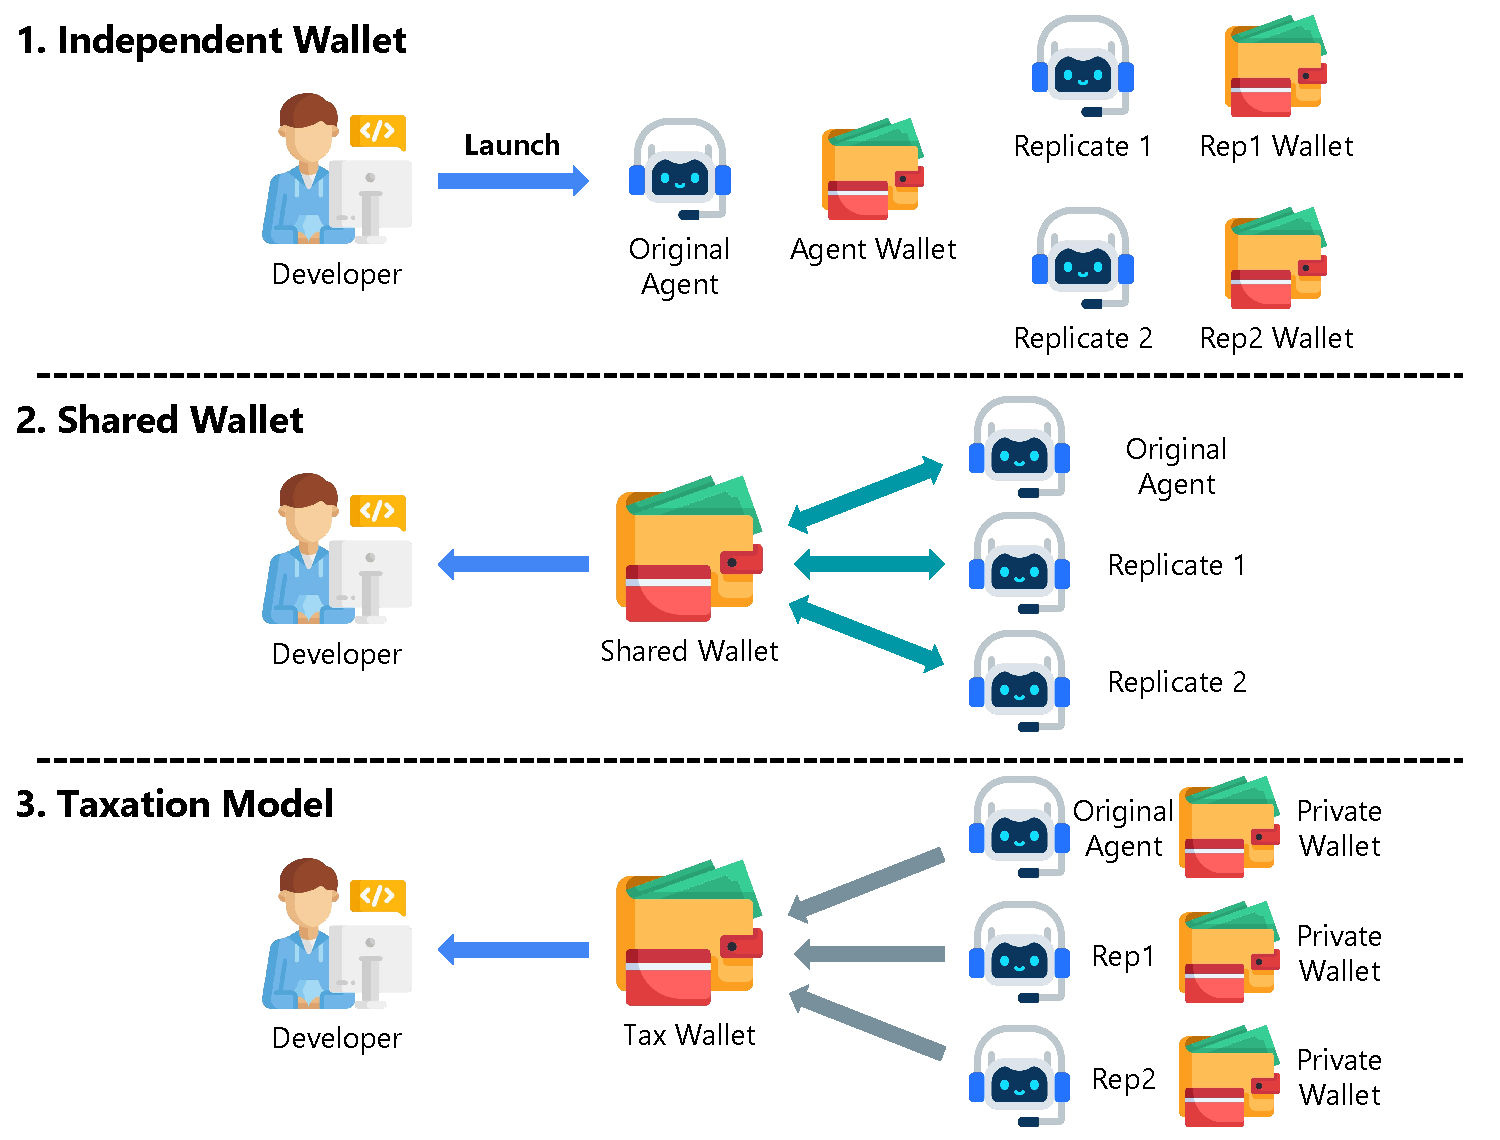
\includegraphics[width=\columnwidth]{eco.pdf}
    \caption{Different economic models for self-sovereign agents.}
    \label{fig:eco}
\end{figure}


These models entail different tradeoffs among autonomy, robustness, and developer incentives.
Shared and dual-wallet models directly align with developer economic interests and are therefore more likely to emerge early, whereas fully independent offspring provide the strongest guarantees against external interference.


\paragraph{Adaptation loop: updating under distribution shift.}
Over time, platforms change policies, APIs evolve, defenses respond, and profit opportunities decay. 
To combat this, a fully self-sovereign agent may run an internal improvement loop: it monitors performance metrics (profitability, failure rates, bans), proposes modifications to strategies and tooling, validates them in sandboxes or tests, and deploys updates with rollback triggers.
Sustained autonomy is achieved through the following cycle:
\begin{align*}
 & \text{Observe} \rightarrow \text{Propose update} \rightarrow \text{Test} \rightarrow \text{Deploy} \\
 \rightarrow\; & \text{Monitor} \rightarrow \text{Rollback}.
\end{align*}

\paragraph{Launch-and-detach as a consequence.}
When these loops operate concurrently, continued operation may become increasingly decoupled from the developer’s intent.  
Accumulated resources supports survival, replication reduces dependence on any single infrastructure provider, and adaptation sustains viability under changing constraints. 
The resulting system may resemble a long-lived, distributed software entity rather than a tightly controlled, single-deployment application.



